%% Creator: Inkscape inkscape 0.48.0, www.inkscape.org
%% PDF/EPS/PS + LaTeX output extension by Johan Engelen, 2010
%% Accompanies image file 'phase_composite.eps' (pdf, eps, ps)
%%
%% To include the image in your LaTeX document, write
%%   \input{<filename>.pdf_tex}
%%  instead of
%%   \includegraphics{<filename>.pdf}
%% To scale the image, write
%%   \def\svgwidth{<desired width>}
%%   \input{<filename>.pdf_tex}
%%  instead of
%%   \includegraphics[width=<desired width>]{<filename>.pdf}
%%
%% Images with a different path to the parent latex file can
%% be accessed with the `import' package (which may need to be
%% installed) using
%%   \usepackage{import}
%% in the preamble, and then including the image with
%%   \import{<path to file>}{<filename>.pdf_tex}
%% Alternatively, one can specify
%%   \graphicspath{{<path to file>/}}
%% 
%% For more information, please see info/svg-inkscape on CTAN:
%%   http://tug.ctan.org/tex-archive/info/svg-inkscape

\begingroup
  \makeatletter
  \providecommand\color[2][]{%
    \errmessage{(Inkscape) Color is used for the text in Inkscape, but the package 'color.sty' is not loaded}
    \renewcommand\color[2][]{}%
  }
  \providecommand\transparent[1]{%
    \errmessage{(Inkscape) Transparency is used (non-zero) for the text in Inkscape, but the package 'transparent.sty' is not loaded}
    \renewcommand\transparent[1]{}%
  }
  \providecommand\rotatebox[2]{#2}
  \ifx\svgwidth\undefined
    \setlength{\unitlength}{228.42889404pt}
  \else
    \setlength{\unitlength}{\svgwidth}
  \fi
  \global\let\svgwidth\undefined
  \makeatother
  \begin{picture}(1,1.91032911)%
    \put(0,0){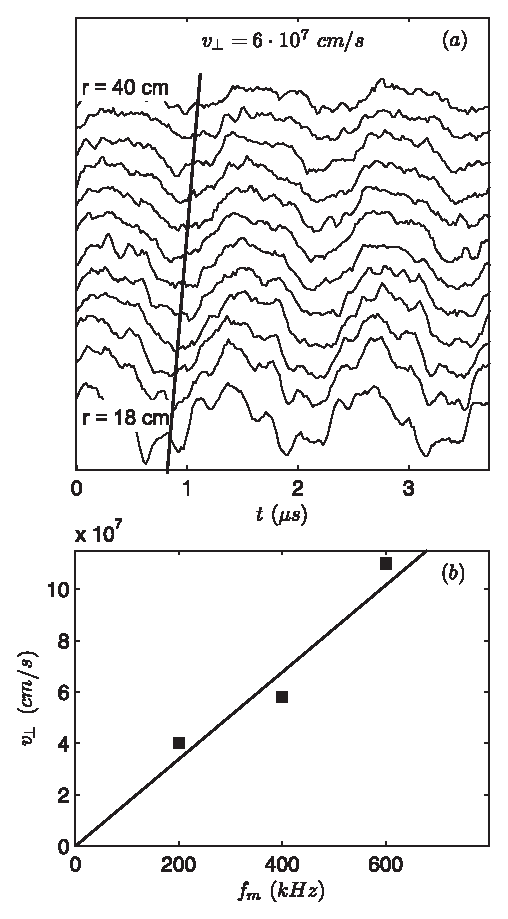
\includegraphics[width=\unitlength]{pics/phase_composite.eps}}%
    \put(0.12,0.868){\color[rgb]{0,0,0}\makebox(0,0)[lb]{\smash{$0$}}}%
    \put(0.353,0.868){\color[rgb]{0,0,0}\makebox(0,0)[lb]{\smash{$1$}}}%
    \put(0.58451047,0.868){\color[rgb]{0,0,0}\makebox(0,0)[lb]{\smash{$2$}}}%
    \put(0.81446356,0.868){\color[rgb]{0,0,0}\makebox(0,0)[lb]{\smash{$3$}}}%
    \put(0.14,1.03){\color[rgb]{0,0,0}\makebox(0,0)[lb]{\smash{$r=18$\,см}}}%
    \put(0.145,1.71){\color[rgb]{0,0,0}\makebox(0,0)[lb]{\smash\bfseries{$r=40$\,см}}}%
    \put(0.5226,0.82){\color[rgb]{0,0,0}\makebox(0,0)[lb]{\smash{$t$\,(мкс)}}}%
    \put(0.9,1.74){\color[rgb]{0,0,0}\makebox(0,0)[lb]{\smash{(a)}}}%

    \put(0.48545375,0.0){\color[rgb]{0,0,0}\makebox(0,0)[lb]{\smash{$f_m$\,(кГц)}}}%
    \put(0.11929763,0.09){\color[rgb]{0,0,0}\makebox(0,0)[lb]{\smash{$0$}}}%
    \put(0.313,0.09){\color[rgb]{0,0,0}\makebox(0,0)[lb]{\smash{$200$}}}%
    \put(0.53,0.09){\color[rgb]{0,0,0}\makebox(0,0)[lb]{\smash{$400$}}}%
    \put(0.748,0.09){\color[rgb]{0,0,0}\makebox(0,0)[lb]{\smash{$600$}}}%
    \put(0.08,0.12){\color[rgb]{0,0,0}\makebox(0,0)[lb]{\smash{$0$}}}%
    \put(0.08,0.232){\color[rgb]{0,0,0}\makebox(0,0)[lb]{\smash{$2$}}}%
    \put(0.08,0.34){\color[rgb]{0,0,0}\makebox(0,0)[lb]{\smash{$4$}}}%
    \put(0.08, 0.448){\color[rgb]{0,0,0}\makebox(0,0)[lb]{\smash{$6$}}}%
    \put(0.08,0.552){\color[rgb]{0,0,0}\makebox(0,0)[lb]{\smash{$8$}}}%
    \put(0.063,0.66){\color[rgb]{0,0,0}\makebox(0,0)[lb]{\smash{$10$}}}%
    \put(0.123,0.77){\color[rgb]{0,0,0}\makebox(0,0)[lb]{\smash{$\times{}10^7$}}}%
    \put(0.037,0.37){\color[rgb]{0,0,0}\rotatebox{90}{\makebox(0,0)[lb]{\smash{$v_\perp$\,(см/с)}}}}%
    \put(0.9,0.68){\color[rgb]{0,0,0}\makebox(0,0)[lb]{\smash{(б)}}}%
  \end{picture}%
\endgroup
